\section*{Section2.4}

\begin{enumerate}
    \item 如图所示二维刚性圆柱, 
    单极子点源声辐射的波数 \(k=40\)  , 
    根据精确格林函数  \(G \) 的解析解, 编程计算:
    
    (1) \(G\) 的空间分布 (空间外边界与坐标原点的距离不小于7倍波长);

    极坐标系下,\(G\)的空间分布如图所示。
    \begin{figure}[htbp]
        \centering
        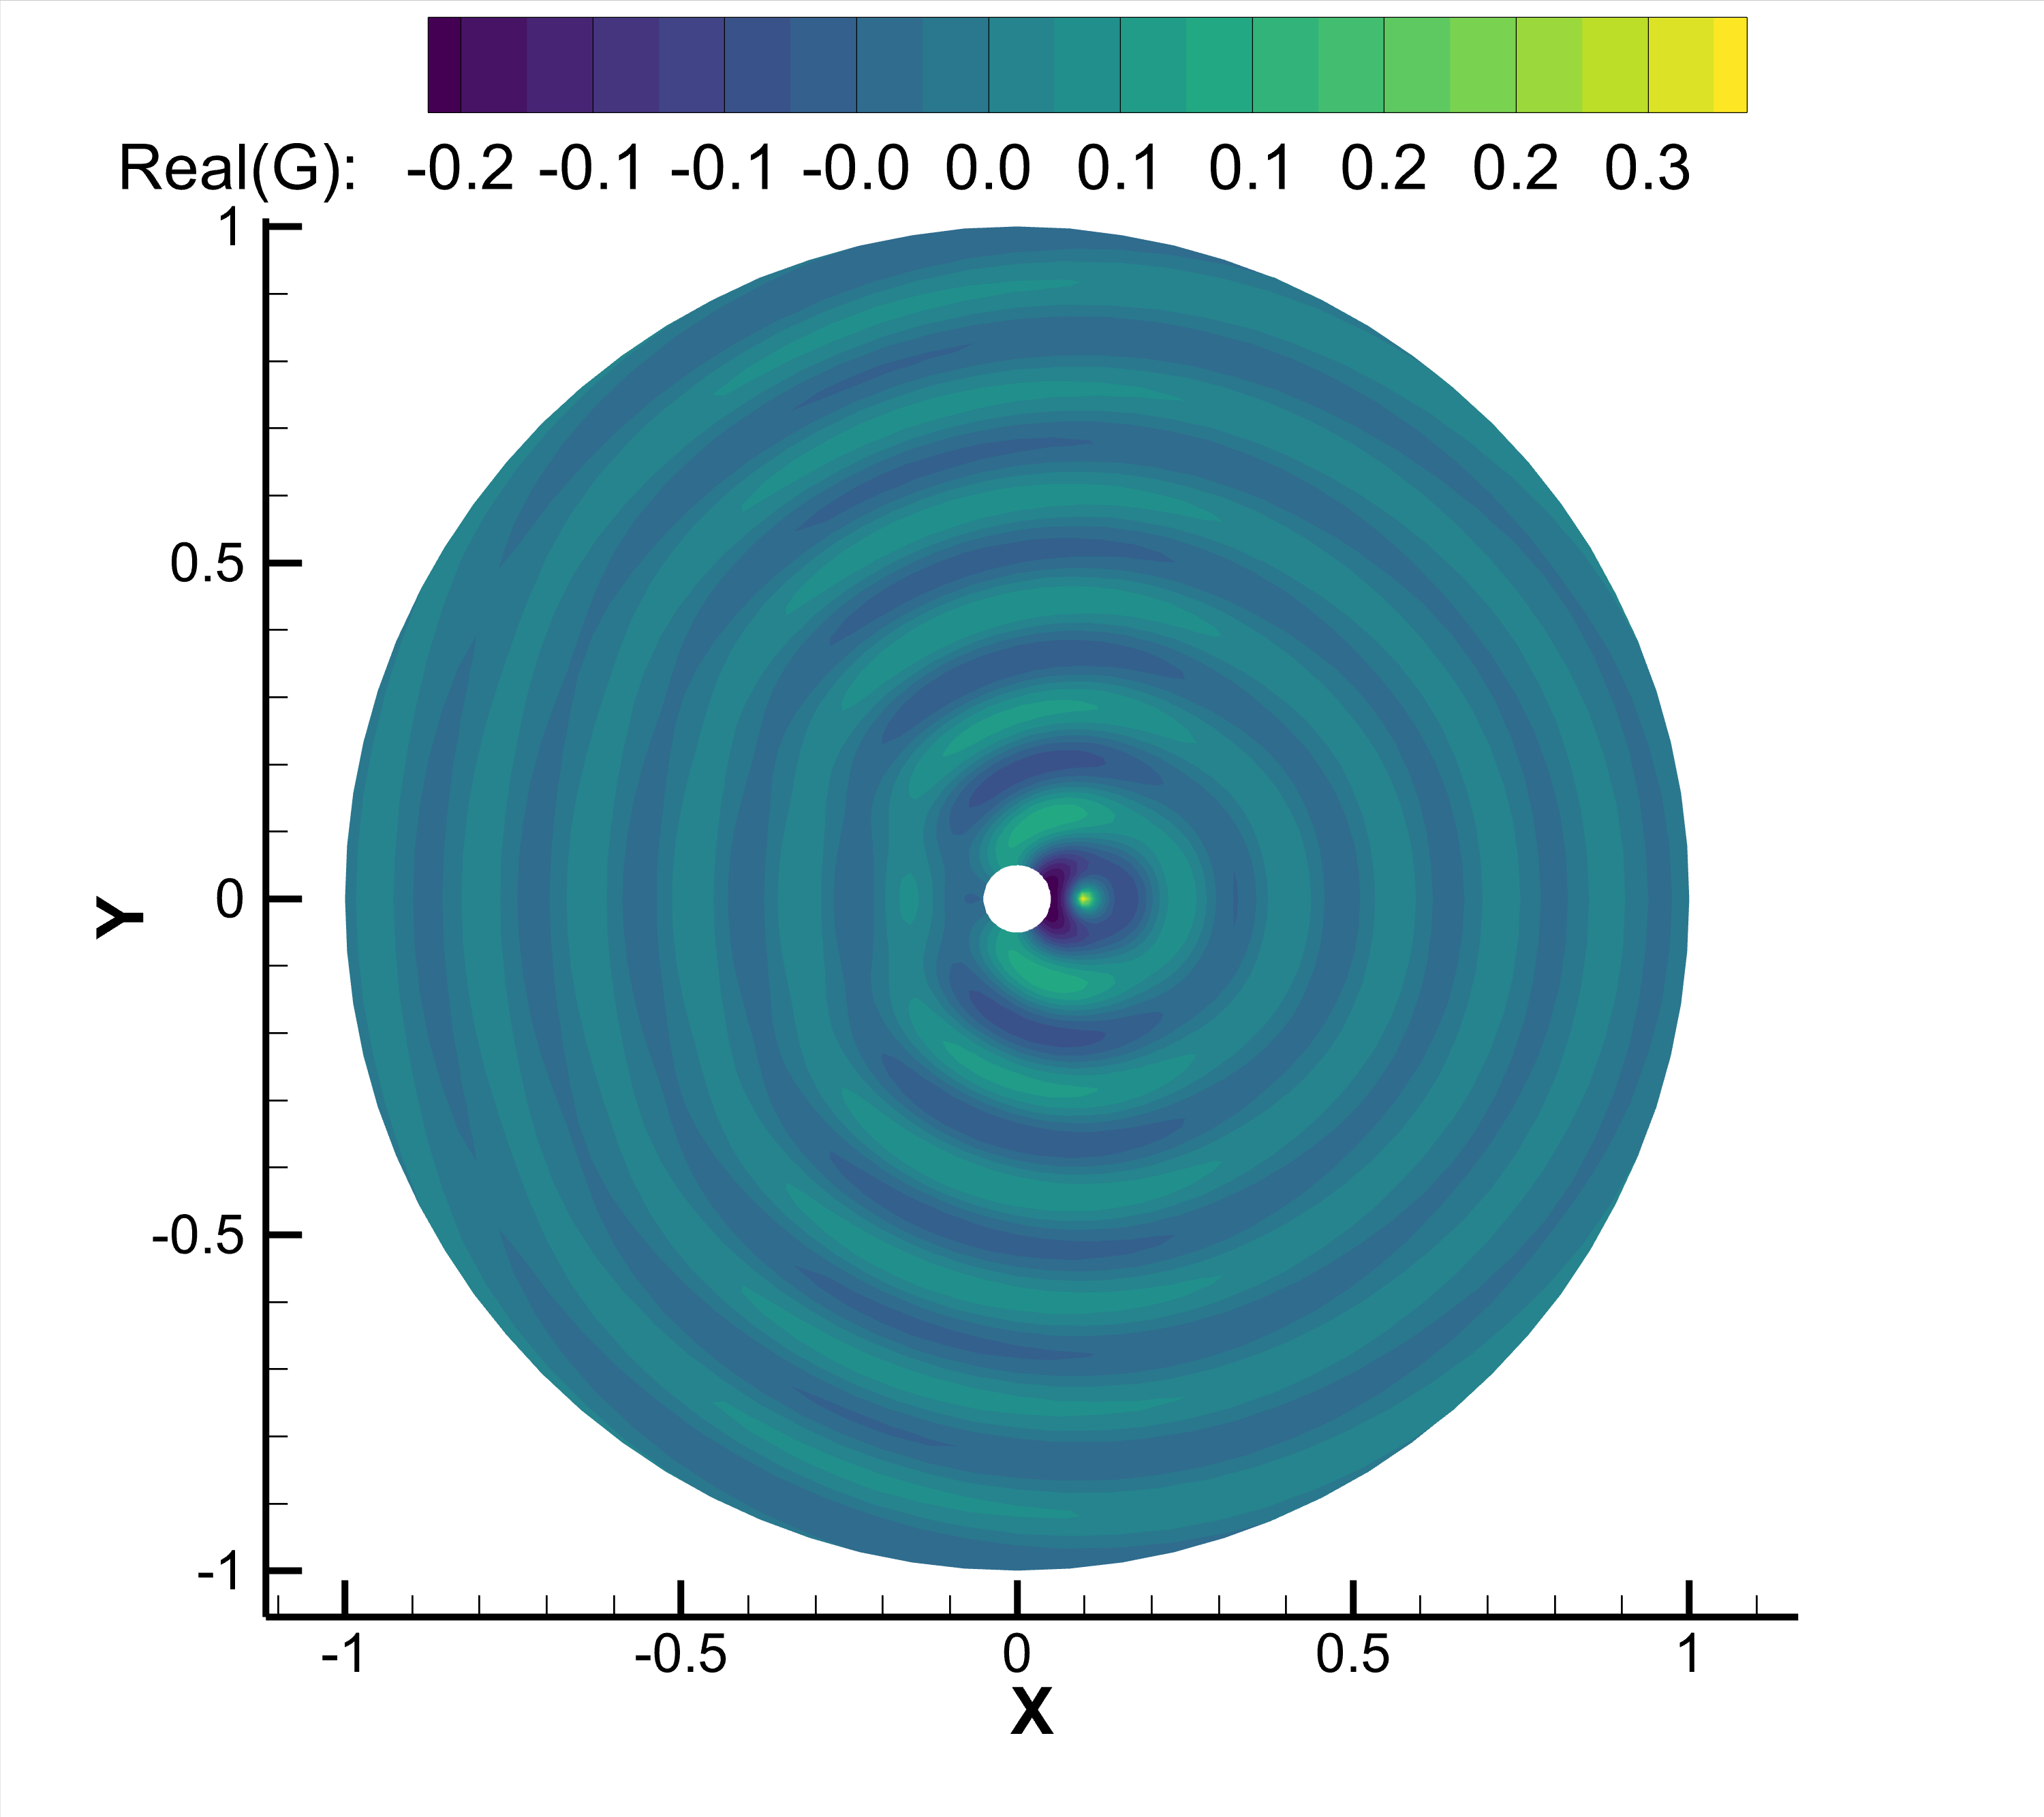
\includegraphics[height=8cm]{image/G.png}
    \end{figure}
    

    (2) \(\partial G / \partial y_{i}\) 的空间分布 ;

    极坐标系下,\(\partial G / \partial r\)的空间分布如图所示。
    \begin{figure}[htbp]
        \centering
        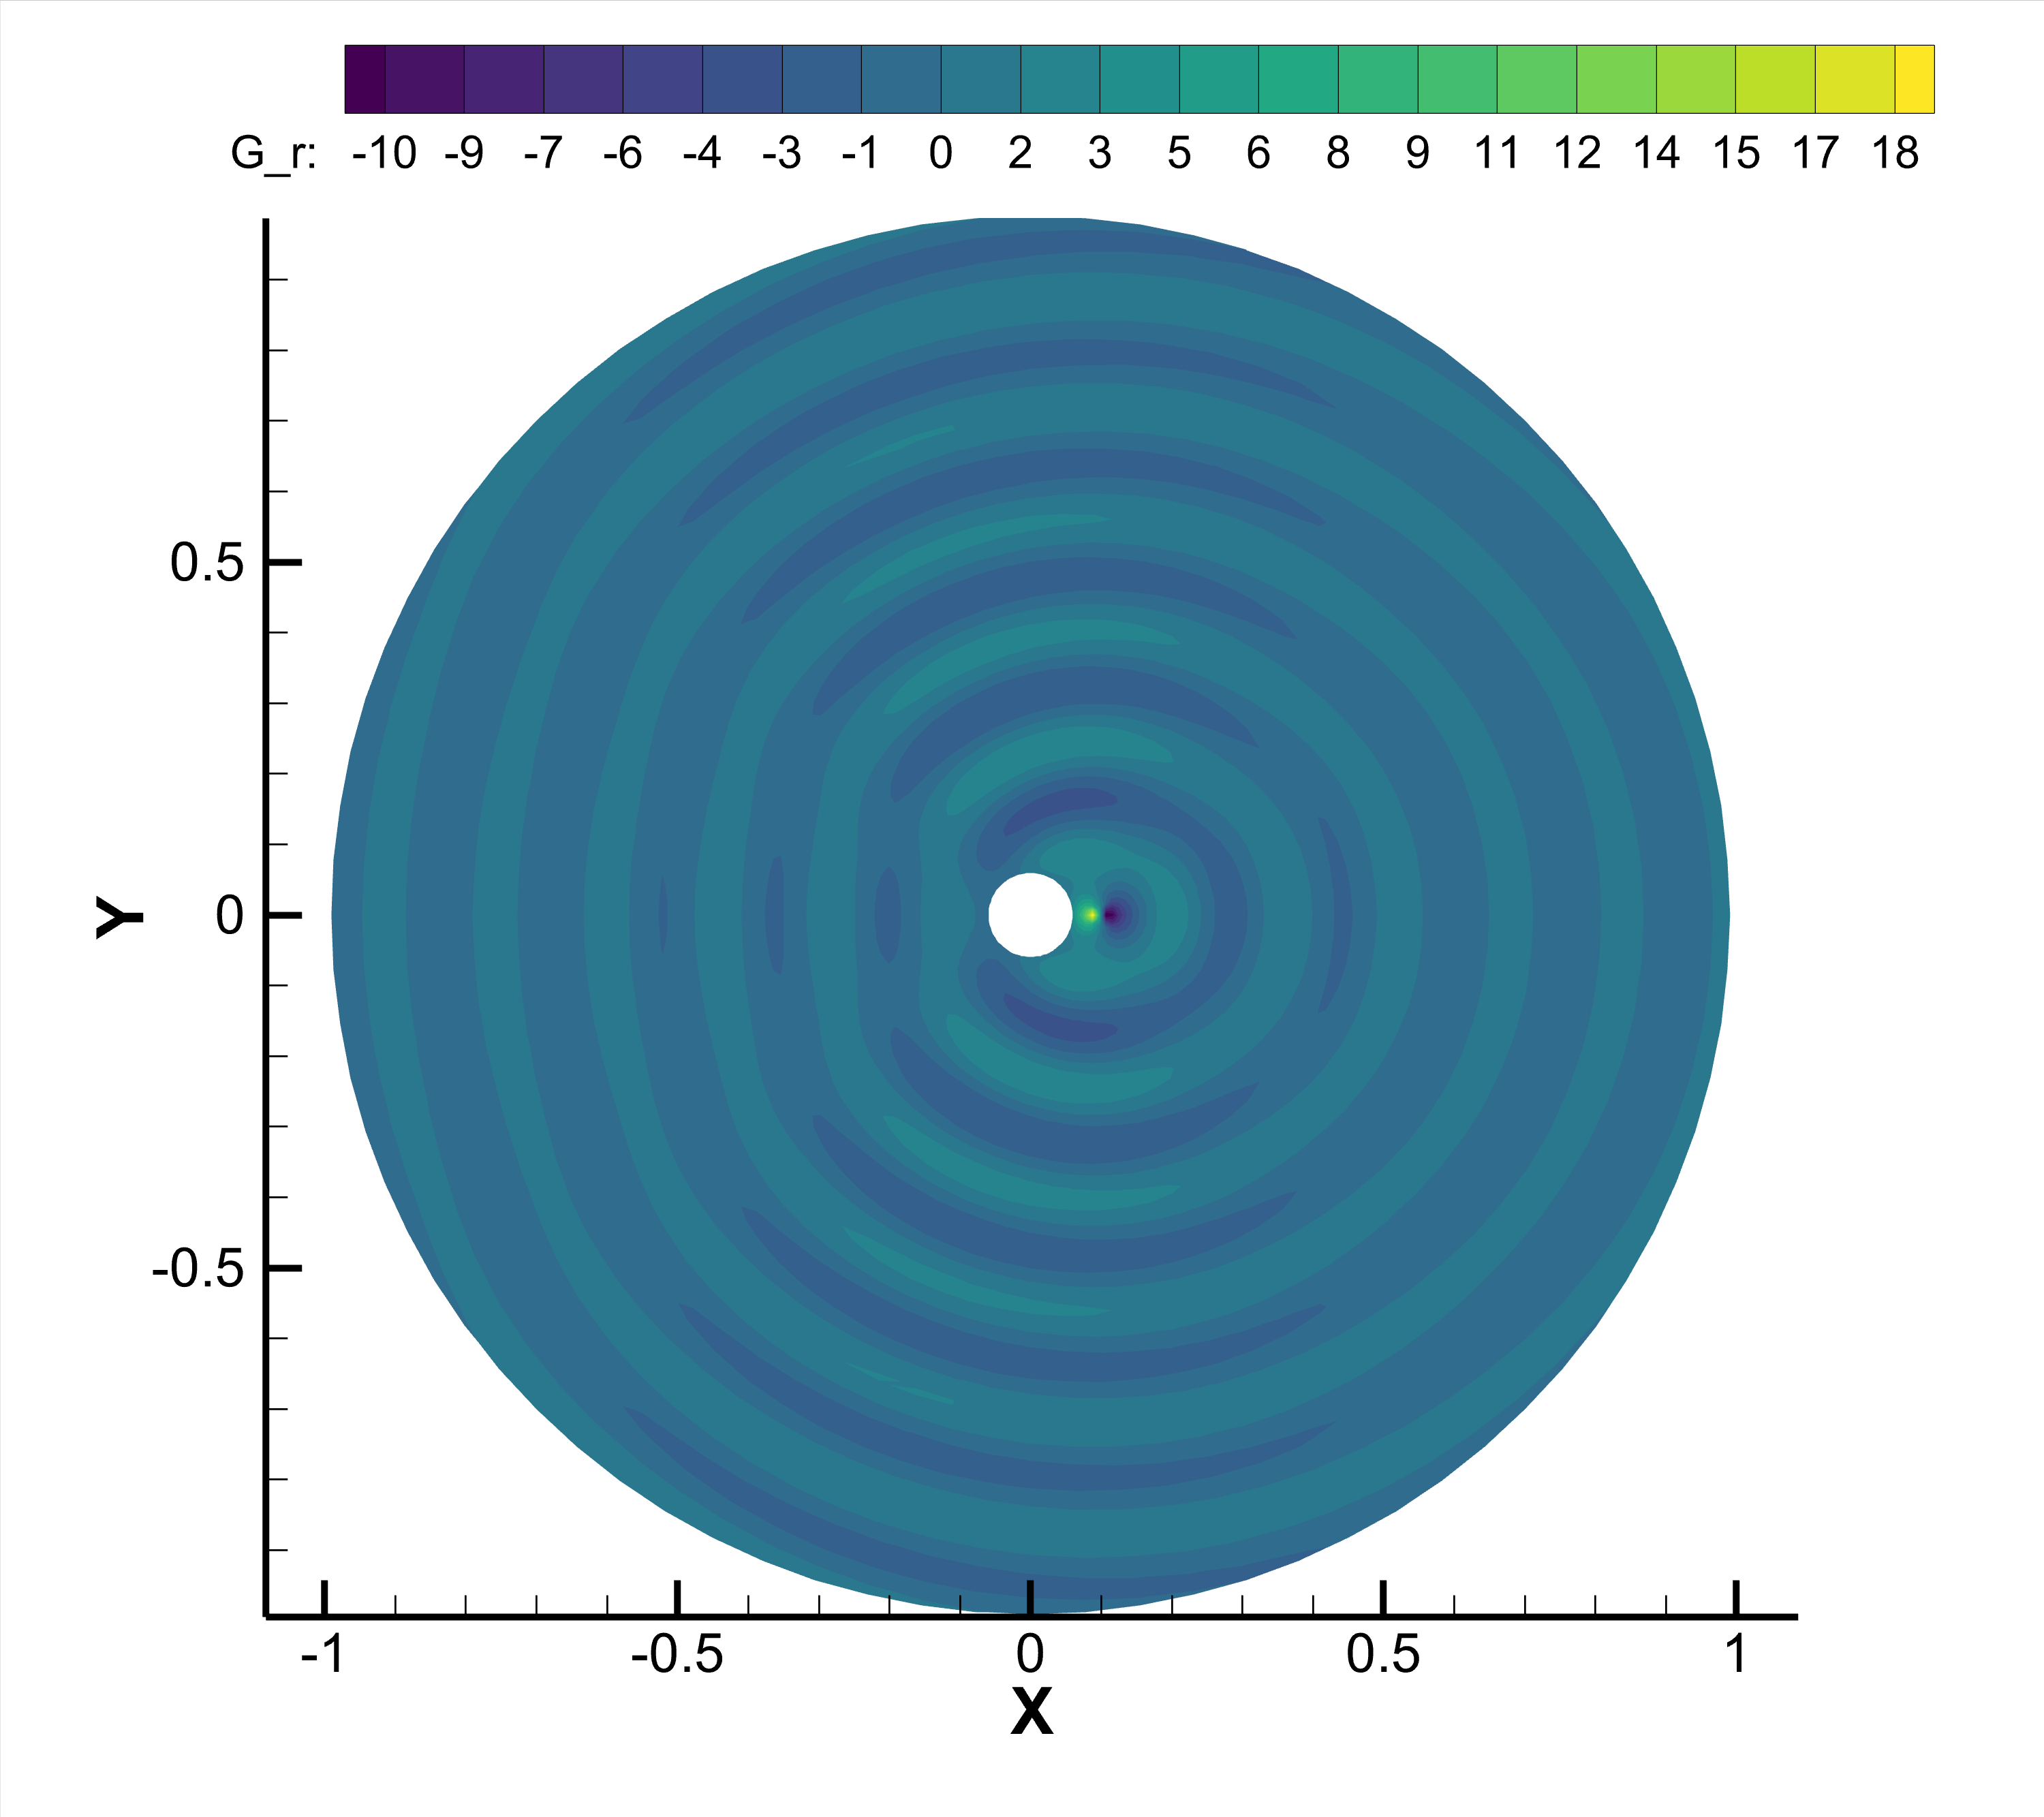
\includegraphics[height=8cm]{image/G_r.png}
    \end{figure}
    
    \clearpage

    (3) \(\partial^{2} G / \partial y_{i} \partial y_{j}\) 的空间分布。
    
    极坐标系下,\(\partial^{2} G / \partial r \partial \theta \)的空间分布如图所示。
    \begin{figure}[htbp]
        \centering
        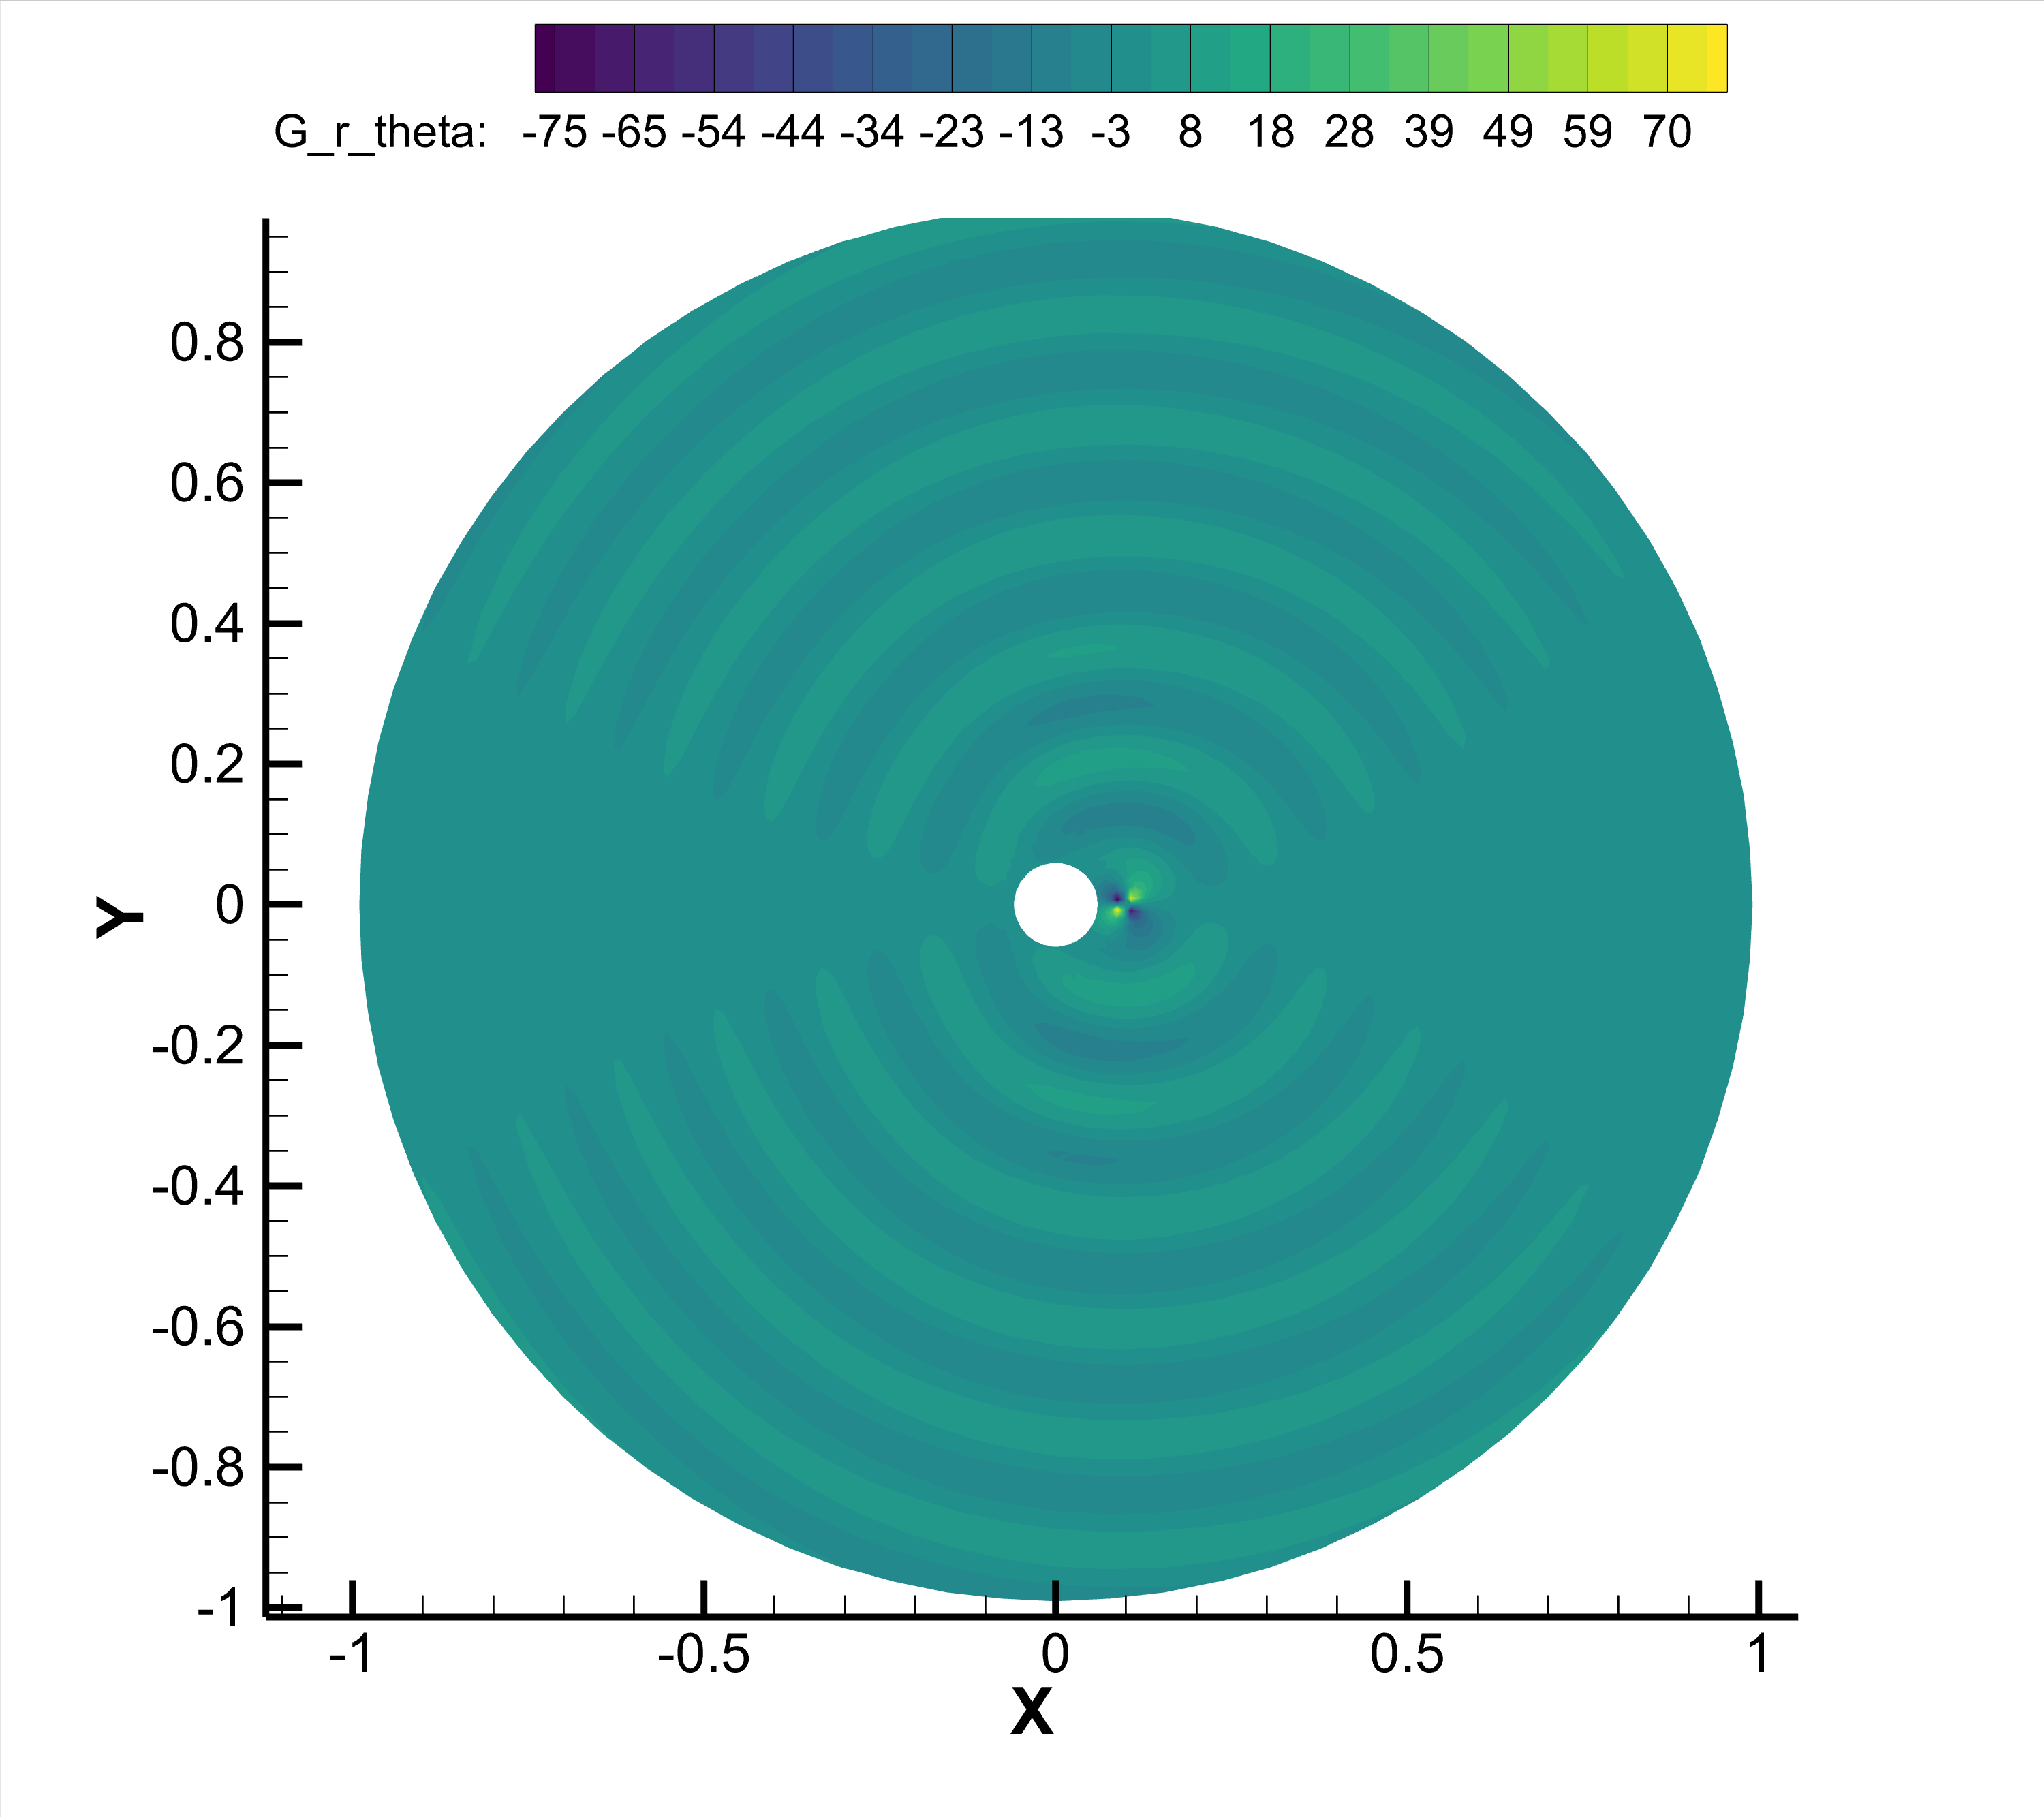
\includegraphics[height=8cm]{image/G_r_theta.png}
    \end{figure}
\end{enumerate}

\clearpage